\section{Existence and uniqueness}

\lecture{14}

\subsection*{A. Independence of choices}

\begin{theorem}
All maximal tori are conjugate. (Recall that we are in the setting of
$\charac k = 0$, $k = \overline{k}$.) That is, if $\at$ and $\at'$ are two
maximal tori of $\g$, then there exists
\[
  g \in \Aut(\g)^0 = \setc{g \in GL(\g)}{g\colon \g \to \g \text{ is a Lie algebra homomorphism}}^0
\]
such that $g\at = \at'$. (Note: $\Aut(\g)$ is itself an algebraic group;
$\Aut(\g)^0$ is the connected component of $1$. Also, for semisimple $\g$,
$\Lie(\Aut \g) = \g$, since every derivation is inner.)
\end{theorem}

The proof is not very hard and involves a little bit of algebraic geometry; we
won't give it.

\begin{theorem}
All positive root systems $R^+$ are conjugate. That is, let $(V, R)$ be a root
system. Let $f_1, f_2\colon V \to \R$ satisfy $f_i(\alpha) \neq 0$ for all
$\alpha \in R$, and define $R^+_{(1)}$, $R^+_{(2)}$ accordingly. There exists a
unique $w \in W$ such that $wR^+_{(1)} = R^+_{(2)}$. (Consequently,
$w\Pi_1 = \Pi_2$ and we get the same Cartan matrix out of the two choices.)
\end{theorem}

The proof is quite easy, but we still won't give it.

\begin{corollary}
$\g$ determines the Cartan matrix, i.e.\ the Dynkin diagram, regardless of the
choices we made.
\end{corollary}

\subsection*{B. Uniqueness}

\begin{theorem}
For $i = 1, 2$, let $\g_i$ be semisimple Lie algebras with Cartan subalgebras
$\at_i$, root systems $R_i$, positive root systems $R_i^+$, simple roots
$\Pi_i$ and Cartan matrices $A_i$. Suppose that, after reordering indices,
$A_1 = A_2$. Then there exists an isomorphism of Lie algebras
$\phi\colon \g_1 \to \g_2$ such that $\phi(\at_1) = \at_2$,
$\phi(R_1) = R_2$, etc.
\end{theorem}

We will not prove this theorem, but we will say more about it.

\subsection*{C. Existence}

\begin{theorem}
Let $A$ be a Cartan matrix. There exists a semisimple Lie algebra whose Cartan
matrix is $A$.
\end{theorem}

\begin{remark}
We already know this for the infinite families, but a nice proof would not be
case-by-case.
\end{remark}

We will now talk about existence and uniqueness.

Let $\g$ be a semisimple Lie algebra, $\g = \at + \bigoplus_{\alpha \in R} \g_\alpha$,
and let the simple roots be $\Pi = \{\alpha_1, \dots, \alpha_l\}$. Choose
\[
  0 \neq E_i \in \g_{\alpha_i}, \quad F_i \in \g_{-\alpha_i}
  \text{ such that } (E_i, F_i)_{\ad} = \frac{2}{(\alpha_i, \alpha_i)}, \qquad
  H_i = \frac{2\nu^{-1}(\alpha_i)}{(\alpha_i, \alpha_i)}.
\]
Define $a_{ij} = (\alpha_i\cv, \alpha_j) = \frac{2(\alpha_i, \alpha_j)}{(\alpha_i, \alpha_i)}$.

We have the following commutation relations:
\begin{itemize}
  \item $[H_i, H_j] = 0$ (the torus commutes);
  \item $[H_i, E_j] = a_{ij}E_j$, since
    \[
      [H_i, E_j] = \alpha_j(H_i)E_j
        = \frac{\alpha_j\bigl(2\nu^{-1}(\alpha_i)\bigr)}{(\alpha_i, \alpha_i)}E_j
        = \frac{2(\alpha_i, \alpha_j)}{(\alpha_i, \alpha_i)}E_j;
    \]
  \item $[H_i, F_j] = -a_{ij}F_j$;
  \item $[E_i, F_j] = 0$ for $i \neq j$, since
    $[E_i, F_j] \in \g_{\alpha_i - \alpha_j}$ and $\alpha_i - \alpha_j \notin R$
    for $\alpha_i, \alpha_j \in \Pi$;
  \item $[E_i, F_i] = H_i$.
\end{itemize}

``Depending on your mood, these are either some of the relations or all of the
relations.'' We will see what this means.

Let $\fn^+ = \bigoplus_{\alpha \in R^+} \g_\alpha$,
$\fn^- = \bigoplus_{\alpha \in -R^+} \g_\alpha$. Then
$\g = \fn^+ + \at + \fn^-$. (Note that $\fn^+$ and $\fn^-$ are subalgebras, but
not ideals, of $\g$.)

\begin{lemma}
The $E_i$ generate $\fn^+$; the $F_i$ generate $\fn^-$; hence the $E_i, F_i$
generate $\g$ as a Lie algebra.
\end{lemma}

\begin{proof}
For a root $\alpha \in R^+$ write $\alpha = \sum k_i\alpha_i$ with
$k_i \in \Z_{\geq 0}$, and define the \emph{height} of $\alpha$ to be
$h(\alpha) = \sum k_i$. We now induct on the height of the root. Recall that if
$\alpha \in R^+$ and $\alpha$ is not simple, then there exists
$\alpha_i \in \Pi$ such that $\alpha - \alpha_i = \beta \in R^+$. By induction,
$\g_\beta$ is generated by the $E_i$. However, then
$\g_\alpha = [\g_\beta, \g_{\alpha_i}]$ is also generated by the $E_i$.

The corresponding claim about the $F_i$ follows immediately by taking $-R^+$ as
the positive roots.

Finally, $[E_i, F_i] = H_i$ and $\setc{H_i}{i = 1, \dots, l}$ is a basis for
$\at$ (recall the simple roots are a basis for $\at^*$).
\end{proof}

Let $A$ be a ``generalised Cartan matrix''. That is, $a_{ii} = 2$,
$a_{ij} = 0$ whenever $a_{ji} = 0$, and $a_{ij} \in \Z_{\leq 0}$ for
$i \neq j$ (but we do not include requirements of positive definiteness). Let
\begin{multline*}
  \gtil = \bigl\langle E_i, F_i, H_i \bigm| [H_i, H_j] = 0,\ [H_i, E_j] = a_{ij}E_j,\\
    [H_i, F_j] = -a_{ij}F_j,\ [E_i, F_j] = 0 \text{ for } i \neq j,\ [E_i, F_i] = H_i\bigr\rangle.
\end{multline*}
Clearly, if $A$ is the Cartan matrix of $\g$, then $\gtil \twoheadrightarrow \g$.
Are these all the relations? Not quite. Let
\[
  \gbar = \gtil\big/\bigl\langle (\ad E_i)^{1 - a_{ij}}E_j = 0,\
    (\ad F_i)^{1 - a_{ij}}F_j = 0 \text{ for } i \neq j\bigr\rangle
\]
(e.g., if $a_{ij} = 0$ then $E_i$ and $E_j$ commute, and if $a_{ij} = -1$ then
$[E_i, [E_i, E_j]] = 0$). These are called the ``Serre relations''.

\begin{remark}
They are called the Serre relations because they were discovered by
Harish-Chandra and Chevalley.
\end{remark}

\begin{exercise}
Check that the Serre relations hold in the classical Lie algebras.
\end{exercise}

\begin{theorem}\leavevmode
\begin{enumerate}
  \item If $A$ is indecomposable, then among the ideals of $\gtil$ meeting
    $\Span\{H_i\}$ trivially there is a unique maximal one, $\fr$. If $A$ is
    symmetrisable (for instance, if $A$ is a Cartan matrix), then $\gbar$ is
    the quotient $\gtil/\fr$, and if moreover $\det A \neq 0$ then $\gbar$ is
    simple. (But it need not be finite-dimensional!)
  \item Hence, if $\g$ is a finite-dimensional semisimple Lie algebra with
    Cartan matrix $A$, then the map $\gtil \to \g$ via $E_i \mapsto E_i$,
    $F_i \mapsto F_i$, $H_i \mapsto H_i$ (where on the left-hand side we have
    the canonical generators of $\gtil$ and on the right-hand side we have the
    elements of the root spaces we found above) factors through $\gbar$ and is
    surjective, so gives an isomorphism $\gbar \cong \g$.
\end{enumerate}
\end{theorem}

The second part of the theorem clearly implies the uniqueness. We also see that
existence is equivalent to the statement
\[
  \gbar \text{ is finite-dimensional} \iff A \text{ is a Cartan matrix}.
\]

\begin{definition}
$\gbar$ (for any $A$) is called a \emph{Kac--Moody algebra} (this time because
they were independently discovered by Kac and Moody).
\end{definition}

Most of the representation theory we will be talking about holds verbatim for
the Kac--Moody algebras. However, note that all we have given for them is a
finite presentation, which is not a very nice object. In particular, the root
spaces of these algebras need not be $1$-dimensional. The dimension of the root
space for any given root is computable but horrible, unless the matrix $A$ is
an affine Dynkin diagram. In that case, the Lie algebra is approximately
$\C c + \g \otimes \C[t, t^{-1}]$.

The Weyl group has a corresponding presentation:

\begin{theorem}[Presentation of the Weyl group]
Write $s_i = s_{\alpha_i}$; then
\[
  W = \bigl\langle s_1, \dots, s_l \bigm| s_i^2 = 1,\ (s_is_j)^{m_{ij}} = 1 \text{ for } i \neq j\bigr\rangle,
\]
where the $m_{ij}$ are defined in terms of the Cartan matrix as follows:
\[
  \begin{array}{c|cccc}
    a_{ij}a_{ji} & 0 & 1 & 2 & 3\\ \hline
    m_{ij} & 2 & 3 & 4 & 6
  \end{array}
\]
\end{theorem}

E.g., if $i$ and $j$ are not connected in the Dynkin diagram then
$s_is_j = s_js_i$, and if they are connected by a single edge, then
$s_is_js_i = s_js_is_j$. These are known as the ``braid relations''. In
$A_{n-1}$ they look like figure~\ref{fig:braid}.

\begin{figure}[!htbp]
\centering
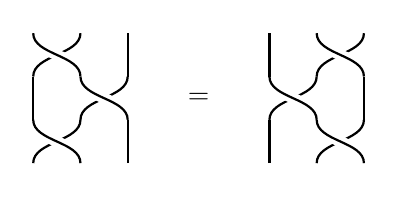
\begin{tikzpicture}[x=0.6cm,y=0.55cm,line width=0.8pt]
  % s_1 s_2 s_1 on strands 0,1,2; each crossing occupies one unit of height
  \newcommand{\cross}[2]{% #1 = left strand position, #2 = bottom height
    \draw (#1,#2) .. controls (#1,#2+0.5) and (#1+1,#2+0.5) .. (#1+1,#2+1);
    \draw[white,line width=4pt] (#1+1,#2) .. controls (#1+1,#2+0.5) and (#1,#2+0.5) .. (#1,#2+1);
    \draw (#1+1,#2) .. controls (#1+1,#2+0.5) and (#1,#2+0.5) .. (#1,#2+1);}
  \begin{scope}
    \cross{0}{0} \draw (2,0)--(2,1);
    \cross{1}{1} \draw (0,1)--(0,2);
    \cross{0}{2} \draw (2,2)--(2,3);
  \end{scope}
  \node at (3.5,1.5) {$=$};
  \begin{scope}[xshift=3cm]
    \cross{1}{0} \draw (0,0)--(0,1);
    \cross{0}{1} \draw (2,1)--(2,2);
    \cross{1}{2} \draw (0,2)--(0,3);
  \end{scope}
\end{tikzpicture}
\caption{Braid relation $s_1s_2s_1 = s_2s_1s_2$ in $A_{n-1}$, drawn on three
strands. We are asserting that the permutations are equal.}
\label{fig:braid}
\end{figure}

\lecture{15}

\begin{exercise}
Check, for each root system, that the relations claimed for the Weyl group do
hold. (This requires checking it for the rank $2$ root systems.) We will not
prove the isomorphism.
\end{exercise}

\begin{remark}
To show existence, we know that $\g = \at + \bigoplus_{\alpha \in R} \g_\alpha$,
so in principle existence should only require picking a basis $E_\alpha$ and
computing $[E_\alpha, E_\beta] = c_{\alpha\beta}E_{\alpha+\beta}$. How hard is
it to write down the $c_{\alpha\beta}$?

For a long time it was thought to be quite hard; however, with the discovery of
the affine Lie algebras, it turned out to be quite easy. We might even get to
doing it for the ADE algebras.
\end{remark}

\begin{remark}
So far the status of existence of a finite-dimensional simple Lie algebra
corresponding to an abstract root system is, for us, as follows: we have shown
that there exists a simple Lie algebra corresponding to each generalised
Cartan matrix, but not that it is finite-dimensional. Suppose that for the
$\gbar$ that we have defined we write
$\gbar = \at + \bigoplus_{\alpha \in R} \gbar_\alpha$ (where the torus comes
from the root system). We can ask two questions: (1) what is the relationship
between $R$ and the root system we started with? (2) What is
$\dim \gbar_\alpha$? While it is true that $W \cdot \Pi \subseteq R$, in
general there is not an equality between them. We call the roots in
$W \cdot \Pi$ ``real roots'', $R^{\mathrm{re}}$; for the real roots,
$\dim \gbar_\alpha = 1$. For finite-dimensional Lie algebras, all roots are
real. If $A$ is an affine Cartan matrix, then the semidefinite nature of it
means that there exists a root of length $0$, unique up to scaling, called the
imaginary root. The imaginary roots are pleasant and describable objects. For
a general, indefinite, Cartan matrix, there exists an algorithm for computing
$\dim \gbar_\alpha$, but the numbers are not very meaningful.
\end{remark}
